\documentclass[crop,tikz]{standalone}% 'crop' is the default for v1.0, before it was 'preview'
\usepackage{tikz,calc,pgfplots}
\usetikzlibrary{calc}
\begin{document}
	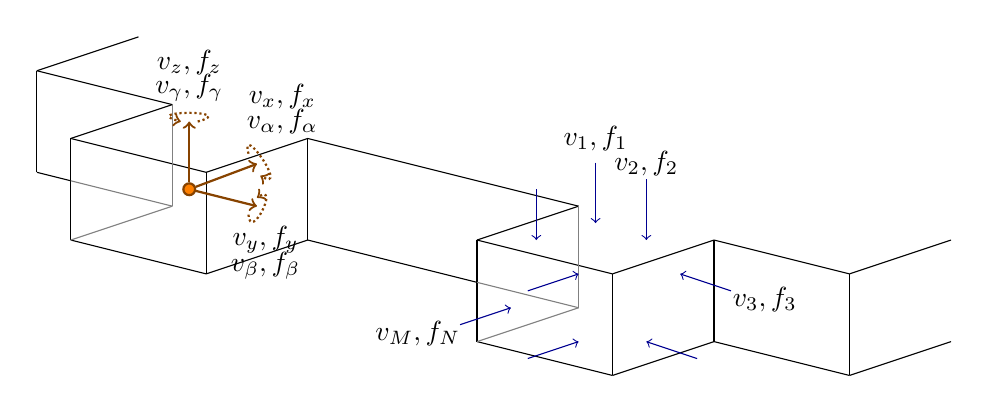
\begin{tikzpicture}[scale=0.43]
% Styles
\tikzstyle{none} = []
\tikzstyle{circle}=[fill={rgb,255: red,255; green,128; blue,0}, draw={rgb,255: red,135; green,67; blue,0}, shape=circle, thick, minimum size=0.15cm, inner sep=0cm]
\tikzstyle{arrow}=[draw={rgb,255: red,135; green,67; blue,0}, ->, thick]
\tikzstyle{greyline}=[-, draw={rgb,255: red,128; green,128; blue,128}]
\tikzstyle{dashedArrow}=[draw={rgb,255: red,135; green,67; blue,0}, densely dotted, thick, ->]
\tikzstyle{new edge style 0}=[draw={rgb,255: red,0; green,0; blue,145}, ->]

\node [style=none] (1) at (-1, 3) {};
\node [style=none] (3) at (-1, 0) {};
\node [style=none] (4) at (-4, 2) {};
\node [style=none] (5) at (-4, -1) {};
\node [style=none] (7) at (0, 1) {};
\node [style=none] (8) at (0, -2) {};
\node [style=none] (9) at (3, 2) {};
\node [style=none] (10) at (3, -1) {};
\node [style=none] (13) at (-5, 4) {};
\node [style=none] (14) at (-5, 1) {};
\node [style=none] (15) at (-2, 5) {};
\node [style=none] (16) at (11, 0) {};
\node [style=none] (17) at (11, -3) {};
\node [style=none] (18) at (8, -1) {};
\node [style=none] (19) at (8, -4) {};
\node [style=none] (20) at (12, -5) {};
\node [style=none] (21) at (12, -2) {};
\node [style=none] (22) at (15, -1) {};
\node [style=none] (23) at (15, -4) {};
\node [style=none] (24) at (19, -2) {};
\node [style=none] (25) at (19, -5) {};
\node [style=none] (26) at (22, -1) {};
\node [style=none] (27) at (22, -4) {};
\node [style=none] (28) at (-4, 0.75) {};
\node [style=none] (29) at (8, -2.25) {};
\node [style=circle] (30) at (-0.5, 0.5) {};
\node [style=none] (31) at (-0.5, 2.5) {};
\node [style=none] (32) at (1.5, 1.25) {};
\node [style=none] (33) at (1.5, 0) {};
\node [style=none] (34) at (-0.25, 2.5) {};
\node [style=none] (35) at (-0.75, 2.5) {};
\node [style=none] (36) at (1.6, 0.9) {};
\node [style=none] (37) at (1.25, 1.55) {};
\node [style=none] (38) at (1.25, -0.25) {};
\node [style=none] (39) at (1.5, 0.25) {};
\node [style=none] (40) at (9.75, -1) {};
\node [style=none] (41) at (9.75, 0.5) {};
\node [style=none] (42) at (11.5, -0.5) {};
\node [style=none, above] (43) at (11.5, 1) {};
\node [style=none] (44) at (13, -1) {};
\node [style=none, above] (45) at (13, 0.5) {};
\node [style=none] (46) at (13, -4) {};
\node [style=none] (47) at (14.5, -4.5) {};
\node [style=none] (48) at (14, -2) {};
\node [style=none] (49) at (15.5, -2.5) {};
\node [style=none] (50) at (11, -4) {};
\node [style=none] (51) at (9.5, -4.5) {};
\node [style=none] (52) at (9, -3) {};
\node [style=none] (53) at (7.5, -3.5) {};
\node [style=none] (54) at (11, -2) {};
\node [style=none] (55) at (9.5, -2.5) {};
\node [style=none] (56) at (11.5, 2) {$v_1,  f_1$};
\node [style=none] (57) at (13, 1) {};
\node [style=none] (58) at (13, 1.25) {$v_2,  f_2$};
\node [style=none] (59) at (11.5, 1.5) {};
\node [style=none] (60) at (11.5, 1.5) {};
\node [style=none] (61) at (11.5, 1.5) {};
\node [style=none] (62) at (11.5, 1.5) {};
\node [style=none] (63) at (16.5, -2.75) {$v_3,  f_3$};
\node [style=none] (64) at (6.25, -3.75) {$v_M,  f_N$};
\node [style=none] (65) at (-0.5, 4.25) {$v_z,  f_z$};
\node [style=none] (66) at (-0.5, 3.5) {$v_\gamma,  f_\gamma$};
\node [style=none] (67) at (2.25, 3.25) {$v_x,  f_x$};
\node [style=none] (69) at (2.25, 2.5) {$v_\alpha,  f_\alpha$};
\node [style=none] (70) at (1.75, -1) {$v_y,  f_y$};
\node [style=none] (71) at (1.75, -1.75) {$v_\beta,  f_\beta$};

\draw (1.center) to (4.center);
\draw (4.center) to (5.center);
\draw (4.center) to (7.center);
\draw (5.center) to (8.center);
\draw [style=greyline] (5.center) to (3.center);
\draw (7.center) to (9.center);
\draw (8.center) to (10.center);
\draw (7.center) to (8.center);
\draw (9.center) to (10.center);
\draw [style=greyline] (1.center) to (3.center);
\draw (13.center) to (15.center);
\draw (13.center) to (14.center);
\draw (13.center) to (1.center);
\draw (9.center) to (16.center);
\draw (16.center) to (18.center);
\draw (18.center) to (19.center);
\draw (21.center) to (18.center);
\draw (20.center) to (19.center);
\draw [style=greyline] (16.center) to (17.center);
\draw [style=greyline] (17.center) to (19.center);
\draw (21.center) to (20.center);
\draw (21.center) to (22.center);
\draw (23.center) to (20.center);
\draw (22.center) to (23.center);
\draw (23.center) to (25.center);
\draw (22.center) to (24.center);
\draw (24.center) to (25.center);
\draw (24.center) to (26.center);
\draw (27.center) to (25.center);
\draw (14.center) to (28.center);
\draw [style=greyline] (28.center) to (3.center);
\draw (10.center) to (29.center);
\draw [style=greyline] (29.center) to (17.center);
\draw [style=arrow] (30) to (31.center);
\draw [style=arrow] (30) to (32.center);
\draw [style=arrow] (30) to (33.center);
\draw [style=dashedArrow, bend right=165, looseness=6.75] (34.center) to (35.center);
\draw [style=dashedArrow, bend right=150, looseness=3.75] (38.center) to (39.center);
\draw [style=dashedArrow, in=-30, out=105, looseness=3.50] (37.center) to (36.center);
\draw [style=new edge style 0] (41.center) to (40.center);
\draw [style=new edge style 0] (43.center) to (42.center);
\draw [style=new edge style 0] (45.center) to (44.center);
\draw [style=new edge style 0] (53.center) to (52.center);
\draw [style=new edge style 0] (47.center) to (46.center);
\draw [style=new edge style 0] (49.center) to (48.center);
\draw [style=new edge style 0] (51.center) to (50.center);
\draw [style=new edge style 0] (55.center) to (54.center);
\end{tikzpicture}
\end{document}